\section{Background}

%%In order to calculate the shutdown dose rate of a nuclear systems,
%%a nuclear inventory must be calculated

\subsection{Nuclear Inventory Analysis}
When a material is irradiated a variety of reactions can happen which
can lead to production of radionuclides. These radionuclides persist
even after a device is shutdown. A nuclear inventory must be known
in order to quantify the photon emission density as a function of time.
The production and destruction of nuclides can be modeled mathematically.
The rate at which a nuclide undergoes a reaction or decay is given by
Equation \ref{total_p_const}.

\begin{equation}\label{total_p_const}
  P_{i \rightarrow j, decay} = P_{i \rightarrow j, reaction } +
  P_{i \rightarrow j, decay}
\end{equation}
The rate in which nuclide i undergoes a reaction is given by equation \ref{reaction_p_const}
\begin{equation}\label{reaction_p_const}
  P_{i \rightarrow j, reaction } =
  \int_{E_{n}} \sigma_{i \rightarrow j}(E_{n})
  \phi_{n}dE_{n}
\end{equation}
where $\sigma_{i \rightarrow j}(E_{n})$ is the microscopic cross
section for the reaction that transforms nuclide $i$ into $j$, and
 $\phi_{n}(E_{n})$ is the neutron flux for energy $E_{n}$.

The production rate constant for the decay process is given by equation
\ref{decay_p_const}

\begin{equation}\label{decay_p_const}
  P_{i \rightarrow j, decay} = \lambda_{i} b_{i \rightarrow j}
\end{equation}
where $\lambda_{i}$ is the decay constant and $b_{i \rightarrow j}$ is
the branching ratio.


\subsection{General Shutdown Dose Rate Workflow}


\begin{figure}[h!]
\begin{centering}
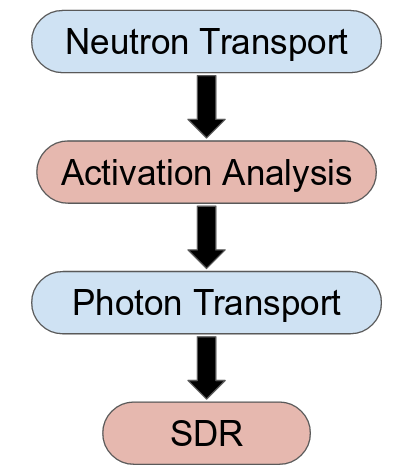
\includegraphics[scale=0.3]{../figs/r2s.png}
% \frame{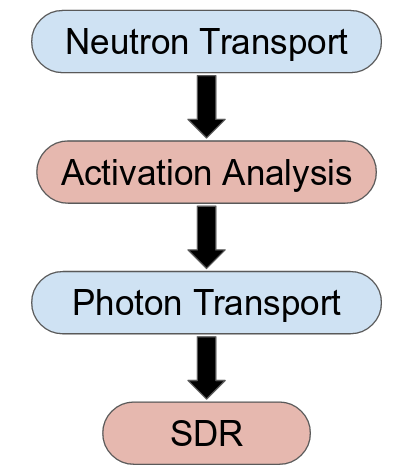
\includegraphics[width=0.30\linewidth, height=4cm]{../figs/r2s.png}}
\caption{General shutdown dose rate workflow}
\label{r2s}
\end{centering}
\end{figure}

\subsection{Shutdown Dose Rate Workflow for High Energy Systems}
The current SDR workflow is seen in Figure \ref{rnucs_r2s}
\begin{figure}[ht!]
\begin{centering}
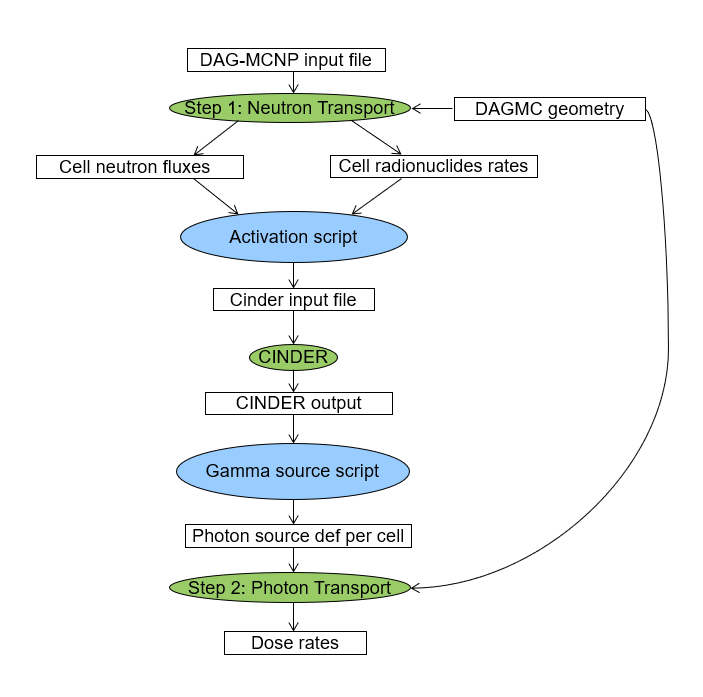
\includegraphics[scale=0.4]{../figs/rnucs_r2s.png}
\caption{Current shut down dose rate workflow for Accelerator systems as used by ORNL}
\label{rnucs_r2s}
\end{centering}
\end{figure}
